\documentclass[12pt]{article}\usepackage[]{graphicx}\usepackage[]{color}
% maxwidth is the original width if it is less than linewidth
% otherwise use linewidth (to make sure the graphics do not exceed the margin)
\makeatletter
\def\maxwidth{ %
  \ifdim\Gin@nat@width>\linewidth
    \linewidth
  \else
    \Gin@nat@width
  \fi
}
\makeatother

\definecolor{fgcolor}{rgb}{0.345, 0.345, 0.345}
\newcommand{\hlnum}[1]{\textcolor[rgb]{0.686,0.059,0.569}{#1}}%
\newcommand{\hlstr}[1]{\textcolor[rgb]{0.192,0.494,0.8}{#1}}%
\newcommand{\hlcom}[1]{\textcolor[rgb]{0.678,0.584,0.686}{\textit{#1}}}%
\newcommand{\hlopt}[1]{\textcolor[rgb]{0,0,0}{#1}}%
\newcommand{\hlstd}[1]{\textcolor[rgb]{0.345,0.345,0.345}{#1}}%
\newcommand{\hlkwa}[1]{\textcolor[rgb]{0.161,0.373,0.58}{\textbf{#1}}}%
\newcommand{\hlkwb}[1]{\textcolor[rgb]{0.69,0.353,0.396}{#1}}%
\newcommand{\hlkwc}[1]{\textcolor[rgb]{0.333,0.667,0.333}{#1}}%
\newcommand{\hlkwd}[1]{\textcolor[rgb]{0.737,0.353,0.396}{\textbf{#1}}}%
\let\hlipl\hlkwb

\usepackage{framed}
\makeatletter
\newenvironment{kframe}{%
 \def\at@end@of@kframe{}%
 \ifinner\ifhmode%
  \def\at@end@of@kframe{\end{minipage}}%
  \begin{minipage}{\columnwidth}%
 \fi\fi%
 \def\FrameCommand##1{\hskip\@totalleftmargin \hskip-\fboxsep
 \colorbox{shadecolor}{##1}\hskip-\fboxsep
     % There is no \\@totalrightmargin, so:
     \hskip-\linewidth \hskip-\@totalleftmargin \hskip\columnwidth}%
 \MakeFramed {\advance\hsize-\width
   \@totalleftmargin\z@ \linewidth\hsize
   \@setminipage}}%
 {\par\unskip\endMakeFramed%
 \at@end@of@kframe}
\makeatother

\definecolor{shadecolor}{rgb}{.97, .97, .97}
\definecolor{messagecolor}{rgb}{0, 0, 0}
\definecolor{warningcolor}{rgb}{1, 0, 1}
\definecolor{errorcolor}{rgb}{1, 0, 0}
\newenvironment{knitrout}{}{} % an empty environment to be redefined in TeX

\usepackage{alltt}

\usepackage{mycommands}

\usepackage{caption}
\usepackage{subcaption}

\usepackage{tikz}
\usetikzlibrary{shadows}
\usetikzlibrary{bayesnet} 
\usepackage[margin=1in]{geometry}

\setlength\parindent{0pt}
\IfFileExists{upquote.sty}{\usepackage{upquote}}{}
\begin{document}
\begin{center}
\Large \underline{Testing Rules Implementation}
\end{center}

\section*{Rule 1}

\begin{figure}[h]
  \centering
  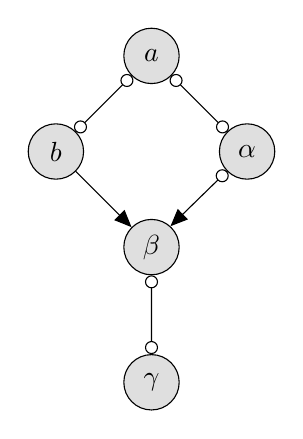
\begin{tikzpicture}[scale=0.33]
% Define nodes
% Top nodes
\node[obs] (a) {$a$};
\node[obs, below left=1 of a] (b) {$b$};
\node[obs, below right=1 of b] (beta) {$\beta$};
\node[obs, below right=1 of a] (alpha) {$\alpha$};
\node[obs, below=1 of beta] (gamma) {$\gamma$};

% Edges
\edge[o-o] {a}{b};
\edge[o-o] {a}{alpha};
\edge[->] {b}{beta};
\edge[o->] {alpha}{beta};
\edge[o-o] {beta}{gamma};
\end{tikzpicture}
  \caption{Testing Rule 1}
  \label{fig:rule1}
\end{figure}

We should see $\beta (3) \rightarrow \gamma (4)$ in the new graph.

\begin{knitrout}
\definecolor{shadecolor}{rgb}{0.969, 0.969, 0.969}\color{fgcolor}\begin{kframe}
\begin{alltt}
\hlkwd{library}\hlstd{(LocalFCI)}
\hlstd{adj.mat1} \hlkwb{<-} \hlkwd{matrix}\hlstd{(}\hlkwd{c}\hlstd{(}\hlnum{0}\hlstd{,}\hlnum{1}\hlstd{,}\hlnum{1}\hlstd{,}\hlnum{0}\hlstd{,}\hlnum{0}\hlstd{,}
                     \hlnum{1}\hlstd{,}\hlnum{0}\hlstd{,}\hlnum{0}\hlstd{,}\hlnum{2}\hlstd{,}\hlnum{0}\hlstd{,}
                     \hlnum{1}\hlstd{,}\hlnum{0}\hlstd{,}\hlnum{0}\hlstd{,}\hlnum{2}\hlstd{,}\hlnum{0}\hlstd{,}
                     \hlnum{0}\hlstd{,}\hlnum{3}\hlstd{,}\hlnum{1}\hlstd{,}\hlnum{0}\hlstd{,}\hlnum{1}\hlstd{,}
                     \hlnum{0}\hlstd{,}\hlnum{0}\hlstd{,}\hlnum{0}\hlstd{,}\hlnum{1}\hlstd{,}\hlnum{0}\hlstd{),}\hlkwc{nrow} \hlstd{=} \hlnum{5}\hlstd{,}\hlkwc{byrow} \hlstd{=} \hlnum{TRUE}\hlstd{)}
\hlstd{adj.mat1.adj} \hlkwb{<-} \hlkwd{rule1}\hlstd{(adj.mat1)}
\end{alltt}
\begin{verbatim}
## Rule 1:
## Orient: 1 *-> 3 o-* 4 as 3 -> 4
\end{verbatim}
\begin{alltt}
\hlkwd{cat}\hlstd{(adj.mat1.adj}\hlopt{$}\hlstd{G[}\hlnum{4}\hlstd{,}\hlnum{5}\hlstd{]}\hlopt{==}\hlnum{2}\hlstd{,}\hlstr{"\textbackslash{}n"}\hlstd{)}
\end{alltt}
\begin{verbatim}
## TRUE
\end{verbatim}
\begin{alltt}
\hlkwd{cat}\hlstd{(adj.mat1.adj}\hlopt{$}\hlstd{G[}\hlnum{5}\hlstd{,}\hlnum{4}\hlstd{]}\hlopt{==}\hlnum{3}\hlstd{,}\hlstr{"\textbackslash{}n"}\hlstd{)}
\end{alltt}
\begin{verbatim}
## TRUE
\end{verbatim}
\end{kframe}
\end{knitrout}

\newpage
\section*{Rule 2}

\begin{figure}[h]
  \centering
  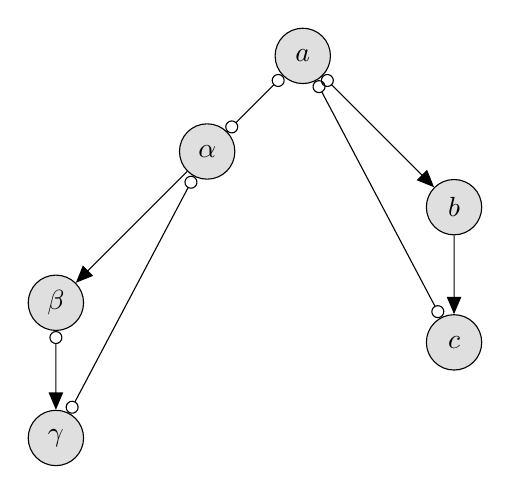
\begin{tikzpicture}[scale=0.33]
% Define nodes
% Top nodes
\node[obs] (a) {$a$};
\node[obs, below right=2 of a] (b) {$b$};
\node[obs, below=1 of b] (c) {$c$};
\node[obs, below left=1 of a] (alpha) {$\alpha$};
\node[obs, below left=2 of alpha] (beta) {$\beta$};
\node[obs, below=1 of beta] (gamma) {$\gamma$};

% Edges
\edge[o->] {a}{b};
\edge[->] {b}{c};
\edge[o-o] {c}{a};
\edge[o-o] {a}{alpha};
\edge[->] {alpha}{beta};
\edge[o->] {beta}{gamma};
\edge[o-o] {gamma}{alpha};
\end{tikzpicture}
  \caption{Testing Rule 2}
  \label{fig:rule2}
\end{figure}

We should see $\alpha (3) \circ \rightarrow \gamma (5)$ and $a (0) \circ \rightarrow c (2)$ in the new graph.

\begin{knitrout}
\definecolor{shadecolor}{rgb}{0.969, 0.969, 0.969}\color{fgcolor}\begin{kframe}
\begin{alltt}
\hlstd{adj.mat2} \hlkwb{<-} \hlkwd{matrix}\hlstd{(}\hlkwd{c}\hlstd{(}\hlnum{0}\hlstd{,}\hlnum{2}\hlstd{,}\hlnum{1}\hlstd{,}\hlnum{1}\hlstd{,}\hlnum{0}\hlstd{,}\hlnum{0}\hlstd{,}
                     \hlnum{1}\hlstd{,}\hlnum{0}\hlstd{,}\hlnum{2}\hlstd{,}\hlnum{0}\hlstd{,}\hlnum{0}\hlstd{,}\hlnum{0}\hlstd{,}
                     \hlnum{1}\hlstd{,}\hlnum{3}\hlstd{,}\hlnum{0}\hlstd{,}\hlnum{0}\hlstd{,}\hlnum{0}\hlstd{,}\hlnum{0}\hlstd{,}
                     \hlnum{1}\hlstd{,}\hlnum{0}\hlstd{,}\hlnum{0}\hlstd{,}\hlnum{0}\hlstd{,}\hlnum{2}\hlstd{,}\hlnum{1}\hlstd{,}
                     \hlnum{0}\hlstd{,}\hlnum{0}\hlstd{,}\hlnum{0}\hlstd{,}\hlnum{3}\hlstd{,}\hlnum{0}\hlstd{,}\hlnum{2}\hlstd{,}
                     \hlnum{0}\hlstd{,}\hlnum{0}\hlstd{,}\hlnum{0}\hlstd{,}\hlnum{1}\hlstd{,}\hlnum{1}\hlstd{,}\hlnum{0}\hlstd{),}\hlkwc{nrow} \hlstd{=} \hlnum{6}\hlstd{,}\hlkwc{byrow} \hlstd{=} \hlnum{TRUE}\hlstd{)}
\hlstd{res} \hlkwb{<-} \hlkwd{rule2}\hlstd{(adj.mat2)}
\end{alltt}
\begin{verbatim}
## Rule 2:
## Orient: 0 *-> 1 -> 2 as: 0 *-> 2
## Rule 2:
## Orient: 3 -> 4 *-> 5 as: 3 *-> 5
\end{verbatim}
\begin{alltt}
\hlkwd{cat}\hlstd{(res}\hlopt{$}\hlstd{G[}\hlnum{1}\hlstd{,}\hlnum{3}\hlstd{]}\hlopt{==}\hlnum{2}\hlstd{,}\hlstr{"\textbackslash{}n"}\hlstd{)}
\end{alltt}
\begin{verbatim}
## TRUE
\end{verbatim}
\begin{alltt}
\hlkwd{cat}\hlstd{(res}\hlopt{$}\hlstd{G[}\hlnum{4}\hlstd{,}\hlnum{6}\hlstd{]}\hlopt{==}\hlnum{2}\hlstd{,}\hlstr{"\textbackslash{}n"}\hlstd{)}
\end{alltt}
\begin{verbatim}
## TRUE
\end{verbatim}
\end{kframe}
\end{knitrout}

\newpage
\section*{Rule 3}

\begin{figure}[h]
  \centering
  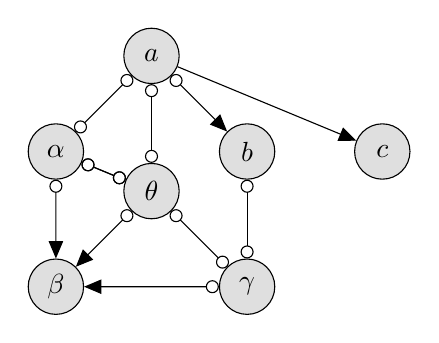
\begin{tikzpicture}[scale=0.33]
% Define nodes
% Top nodes
\node[obs] (a) {$a$};
\node[obs, below right=1 of a] (b) {$b$};
\node[obs, right=1 of b] (c) {$c$};
\node[obs, below left=1 of a] (alpha) {$\alpha$};
\node[obs, below=1 of a] (theta) {$\theta$};
\node[obs, below=1 of alpha] (beta) {$\beta$};
\node[obs, below right=1 of theta] (gamma) {$\gamma$};

% Edges
\edge[o->] {a}{b};
\edge[<-] {c}{a};
\edge[o-o] {a}{alpha};
\edge[o-o] {alpha}{theta};
\edge[o-o] {alpha}{theta};
\edge[o->] {alpha}{beta};
\edge[o-o] {b}{gamma};
\edge[o-o] {theta}{gamma};
\edge[o-o] {theta}{a};
\edge[o->] {theta}{beta};
\edge[o->] {gamma}{beta};
\end{tikzpicture}
  \caption{Testing Rule 3}
  \label{fig:rule3}
\end{figure}

We should see $\theta(6) \circ \rightarrow \beta (4)$
\begin{knitrout}
\definecolor{shadecolor}{rgb}{0.969, 0.969, 0.969}\color{fgcolor}\begin{kframe}
\begin{alltt}
\hlstd{adj.mat3} \hlkwb{<-} \hlkwd{matrix}\hlstd{(}\hlkwd{c}\hlstd{(}\hlnum{0}\hlstd{,}\hlnum{2}\hlstd{,}\hlnum{2}\hlstd{,}\hlnum{1}\hlstd{,}\hlnum{0}\hlstd{,}\hlnum{0}\hlstd{,}\hlnum{1}\hlstd{,}
                     \hlnum{1}\hlstd{,}\hlnum{0}\hlstd{,}\hlnum{0}\hlstd{,}\hlnum{0}\hlstd{,}\hlnum{0}\hlstd{,}\hlnum{1}\hlstd{,}\hlnum{0}\hlstd{,}
                     \hlnum{3}\hlstd{,}\hlnum{0}\hlstd{,}\hlnum{0}\hlstd{,}\hlnum{0}\hlstd{,}\hlnum{0}\hlstd{,}\hlnum{0}\hlstd{,}\hlnum{0}\hlstd{,}
                     \hlnum{1}\hlstd{,}\hlnum{0}\hlstd{,}\hlnum{0}\hlstd{,}\hlnum{0}\hlstd{,}\hlnum{2}\hlstd{,}\hlnum{0}\hlstd{,}\hlnum{1}\hlstd{,}
                     \hlnum{0}\hlstd{,}\hlnum{0}\hlstd{,}\hlnum{0}\hlstd{,}\hlnum{1}\hlstd{,}\hlnum{0}\hlstd{,}\hlnum{1}\hlstd{,}\hlnum{1}\hlstd{,}
                     \hlnum{0}\hlstd{,}\hlnum{1}\hlstd{,}\hlnum{0}\hlstd{,}\hlnum{0}\hlstd{,}\hlnum{2}\hlstd{,}\hlnum{0}\hlstd{,}\hlnum{1}\hlstd{,}
                     \hlnum{1}\hlstd{,}\hlnum{0}\hlstd{,}\hlnum{0}\hlstd{,}\hlnum{1}\hlstd{,}\hlnum{1}\hlstd{,}\hlnum{1}\hlstd{,}\hlnum{0}\hlstd{),}\hlkwc{nrow} \hlstd{=} \hlnum{7}\hlstd{,}\hlkwc{byrow} \hlstd{=} \hlnum{TRUE}\hlstd{)}
\hlstd{res} \hlkwb{<-} \hlkwd{rule3}\hlstd{(adj.mat3)}
\end{alltt}
\begin{verbatim}
## Rule 3:
## Orient: 6 *-> 4
\end{verbatim}
\begin{alltt}
\hlkwd{cat}\hlstd{(res}\hlopt{$}\hlstd{G[}\hlnum{7}\hlstd{,}\hlnum{5}\hlstd{]}\hlopt{==}\hlnum{2}\hlstd{,}\hlstr{"\textbackslash{}n"}\hlstd{)}
\end{alltt}
\begin{verbatim}
## TRUE
\end{verbatim}
\end{kframe}
\end{knitrout}

\newpage
\section*{Rule 4}

\begin{figure}[h]
  \centering
  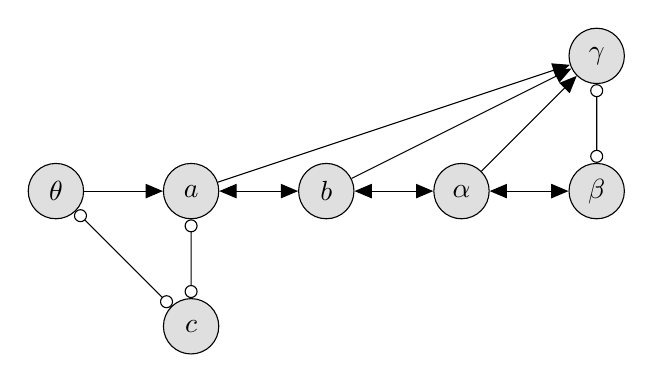
\begin{tikzpicture}[scale=0.33]
% Define nodes
\node[obs] (theta) {$\theta$};
\node[obs, right=1 of theta] (a) {$a$};
\node[obs, right=1 of a] (b) {$b$};
\node[obs, below=1 of a] (c) {$c$};
\node[obs, right=1 of b] (alpha) {$\alpha$};
\node[obs, right=1 of alpha] (beta) {$\beta$};
\node[obs, above=1 of beta] (gamma) {$\gamma$};

% Edges
\edge[->] {theta}{a};
\edge[o-o] {theta}{c};
\edge[o-o] {a}{c};
\edge[<->] {a}{b};
\edge[<->] {b}{alpha};
\edge[<->] {alpha}{beta};
\edge[->] {a}{gamma};
\edge[->] {b}{gamma};
\edge[->] {alpha}{gamma};
\edge[o-o] {beta}{gamma};
\end{tikzpicture}
  \caption{Testing Rule 3}
  \label{fig:rule3}
\end{figure}

If we let $\beta \in $ SepSet($\theta$,$\gamma$), then we should have $\beta (4) \rightarrow \gamma (5)$.
\begin{knitrout}
\definecolor{shadecolor}{rgb}{0.969, 0.969, 0.969}\color{fgcolor}\begin{kframe}
\begin{alltt}
\hlstd{adj.mat4} \hlkwb{<-} \hlkwd{matrix}\hlstd{(}\hlkwd{c}\hlstd{(}\hlnum{0}\hlstd{,}\hlnum{2}\hlstd{,}\hlnum{1}\hlstd{,}\hlnum{0}\hlstd{,}\hlnum{0}\hlstd{,}\hlnum{2}\hlstd{,}\hlnum{3}\hlstd{,}
                     \hlnum{2}\hlstd{,}\hlnum{0}\hlstd{,}\hlnum{0}\hlstd{,}\hlnum{2}\hlstd{,}\hlnum{0}\hlstd{,}\hlnum{2}\hlstd{,}\hlnum{0}\hlstd{,}
                     \hlnum{3}\hlstd{,}\hlnum{0}\hlstd{,}\hlnum{0}\hlstd{,}\hlnum{0}\hlstd{,}\hlnum{3}\hlstd{,}\hlnum{0}\hlstd{,}\hlnum{1}\hlstd{,}
                     \hlnum{0}\hlstd{,}\hlnum{2}\hlstd{,}\hlnum{0}\hlstd{,}\hlnum{0}\hlstd{,}\hlnum{2}\hlstd{,}\hlnum{2}\hlstd{,}\hlnum{0}\hlstd{,}
                     \hlnum{0}\hlstd{,}\hlnum{0}\hlstd{,}\hlnum{2}\hlstd{,}\hlnum{2}\hlstd{,}\hlnum{0}\hlstd{,}\hlnum{1}\hlstd{,}\hlnum{0}\hlstd{,}
                     \hlnum{3}\hlstd{,}\hlnum{3}\hlstd{,}\hlnum{0}\hlstd{,}\hlnum{3}\hlstd{,}\hlnum{1}\hlstd{,}\hlnum{0}\hlstd{,}\hlnum{0}\hlstd{,}
                     \hlnum{2}\hlstd{,}\hlnum{0}\hlstd{,}\hlnum{1}\hlstd{,}\hlnum{0}\hlstd{,}\hlnum{0}\hlstd{,}\hlnum{0}\hlstd{,}\hlnum{0}\hlstd{),}\hlkwc{nrow} \hlstd{=} \hlnum{7}\hlstd{,}\hlkwc{byrow} \hlstd{=} \hlnum{TRUE}\hlstd{)}
\hlstd{S} \hlkwb{<-} \hlkwd{create_conditioning_sets_efficient_cpp2}\hlstd{(}\hlkwd{seq}\hlstd{(}\hlnum{0}\hlstd{,}\hlnum{6}\hlstd{))}
\hlstd{nodes} \hlkwb{<-} \hlkwd{c}\hlstd{(}\hlstr{"a"}\hlstd{,}\hlstr{"b"}\hlstd{,}\hlstr{"c"}\hlstd{,}\hlstr{"alpha"}\hlstd{,}\hlstr{"beta"}\hlstd{,}\hlstr{"gamma"}\hlstd{,}\hlstr{"theta"}\hlstd{)}
\hlstd{S[[}\hlstr{"6"}\hlstd{]][[}\hlstr{"5"}\hlstd{]]} \hlkwb{<-} \hlnum{4}
\hlstd{S[[}\hlstr{"5"}\hlstd{]][[}\hlstr{"6"}\hlstd{]]} \hlkwb{<-} \hlnum{4}

\hlkwd{rule4}\hlstd{(adj.mat4,S)}
\end{alltt}
\begin{verbatim}
## Potential beta: 2 | Potential gamma: 0
## Potential beta: 2 | Potential gamma: 6
## Potential beta: 4 | Potential gamma: 5 | Potential alpha: 3
## Potential values: 1
## Creating path list
## New Path: 3 1
## mpath: 3 1
## Potential values for the path: 0
## Size of old path list: 1
## Size of new path list: 2
## Path 0: 3 1
## Path 1: 3 1 0
## mpath: 3 1 0
## Potential values for the path: 6
## Size of old path list: 2
## Size of new path list: 3
## Path 0: 3 1
## Path 1: 3 1 0
## Path 2: 3 1 0 6
## mpath: 3 1 0 6
## Minimum Discriminating Path: 6 0 1 3 4 5
## Checking separation...finished
## 
## Rule4
## There is a discriminating path between6 and 5 for 4 and 4 is in the SepSet of 5 and 6. Orient: 4 -> 5
## 
## Potential beta: 6 | Potential gamma: 2
\end{verbatim}
\end{kframe}
\end{knitrout}


\end{document}

